%----------------------------------------------------------------------------------------
%	PACKAGES AND OTHER DOCUMENT CONFIGURATIONS
%----------------------------------------------------------------------------------------
\documentclass[fleqn,9 pt]{SelfArx} % Document font size and equations flushed left

% Decrease margins
%\addtolength{\oddsidemargin}{-0.3 in}
%\addtolength{\evensidemargin}{0 in}
%\addtolength{\textwidth}{0.8 in}
%\addtolength{\topmargin}{-0.5 in}
%\addtolength{\textheight}{1 in}

\usepackage[english]{babel} % Specify a different language here - english by default
\usepackage{lipsum} % Required to insert dummy text. To be removed otherwise
\usepackage{listings}
\usepackage{lipsum}  
\usepackage{caption}

%----------------------------------------------------------------------------------------
%	COLUMNS
%----------------------------------------------------------------------------------------
\setlength{\columnsep}{0.55cm} % Distance between the two columns of text
\setlength{\fboxrule}{0.75pt} % Width of the border around the abstract
%----------------------------------------------------------------------------------------
%	COLORS
%----------------------------------------------------------------------------------------
\definecolor{color1}{RGB}{0,0,90} % Color of the article title and sections
\definecolor{color2}{RGB}{0,20,20} % Color of the boxes behind the abstract and headings

%----------------------------------------------------------------------------------------
%	HYPERLINKS
%----------------------------------------------------------------------------------------
\usepackage{hyperref} % Required for hyperlinks
\hypersetup{hidelinks,colorlinks,breaklinks=true,urlcolor=color2,citecolor=color1,linkcolor=color1,bookmarksopen=false,pdftitle={Title},pdfauthor={Author}}

%----------------------------------------------------------------------------------------
%	ARTICLE INFORMATION
%----------------------------------------------------------------------------------------
\JournalInfo{Mini-project 1 - CS-433 - Pattern Classification and Machine Learning} % Journal information
\Archive{\today} % Additional notes (e.g. copyright, DOI, review/research article)

%%%%% dumb test
\usepackage[english]{babel}
\usepackage{blindtext}

\PaperTitle{The Higgs boson machine learning challenge} % Article title

\Authors{Bruno Magalhaes\textsuperscript{1}, Marie Drieghe\textsuperscript{2}, Nicolas Casademont \textsuperscript{3}} % Authors
\affiliation{\textbf{Email (SCIPER):} \hspace{0.2cm} \textsuperscript{1} bruno.magalhaes@epfl.ch (212079) \hspace{0.2cm} \textsuperscript{2} marie.drieghe@epfl.ch (273688) \hspace{0.2cm} \textsuperscript{3} nicolas.casademont@epfl.ch (223485)}

\Keywords{}
%Keyword1 --- Keyword2 --- Keyword3

\newcommand{\keywordname}{Keywords} % Defines the keywords heading name

%to allow overlapping
\usepackage[percent]{overpic}
\usepackage[]{algorithmic,algorithm2e}

%to allow \figures right below text 
\usepackage{float}

%---------- ABSTRACT

\Abstract{ \small
Decay signatures of proton-proton collisions led to the discovery of the Higgs Boson. This new particle was discovered by analysing areas with a significant amount of unknown events (signals) against others that contain known ones (background). To tackle the challenge, we present a Machine Learning (ML) algorithm for the classification of these areas. Our algorithm reaches more than 80\% accuracy by combing feature engineering and logistic regression. Due to the high-dimensionality of the solution, we perform iterative stepping via the stochastic gradient descent method. We detail a set of pre-processing methods that allow for shorter data set, smaller dimensionality, faster execution time, filtering of outliers, and imputation of missing values.
}

\begin{document}
\begin{sloppypar} %allows line breaks in \texttt{---} section

\flushbottom % Makes all text pages the same height
\maketitle % Print the title and abstract box
%\tableofcontents % Print the contents section
\thispagestyle{empty} % Removes page numbering from the first page

We present the sequence of pre-processing filtering steps tested in Section \ref{sec-pre-proc}, where we explain their rationale and detail the results. The data after filtering is then used in the Machine Learning methods described in Section \ref{sec-ML} to create a classification model. Results and final remarks are detailed in Section \ref{sec-results}.

\section{Data Augmentation}
\label{sec-pre-proc}

\paragraph{1. Rotation of input images with non-orthogonal roads} We increased the number of input images from $100$ to $148$ by rotating $90 \deg$, $180 \deg$ and $270 \deg$ the (16) training images that are not composed only of non-horizontal and non-vertical roads. This feature is activated by the flag \texttt{DATA\_AUGMENTATION}.

\paragraph{2. Patches from concatenation points} We increase by almost two-fold the number of patches per training image by performing extraction of all patches of size \texttt{IMG\_PATCH\_SIZE} that are placed at every \texttt{IMG\_PATCH\_SIZE/2} interval. This feature is activated by the flag \texttt{ADD\_INTERCALATED\_PATCHES}. In practice, it extracts patches with the corners at the mid-point positions of previously extracted patches, as displayed below:

\begin{figure}[H]
\centering
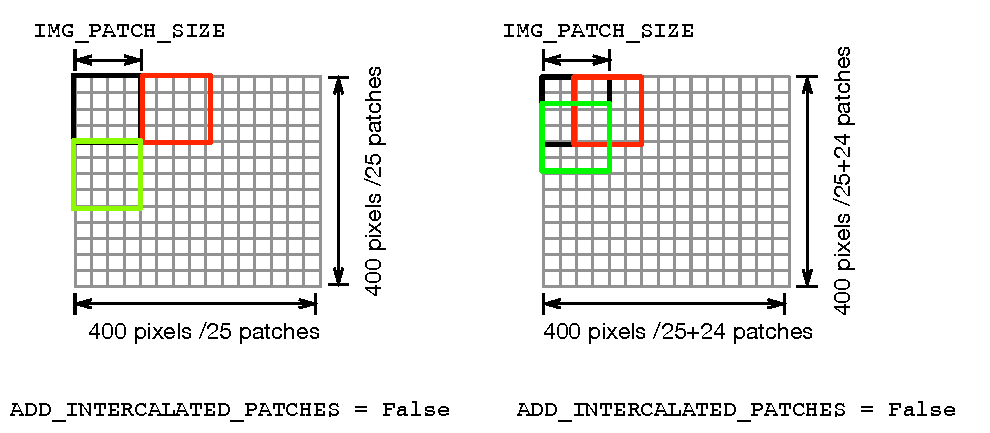
\includegraphics[width=0.47\textwidth]{figures/ADD_INTERCALATED_PATCHES.pdf}
\caption{\small The collection of patches by stepping \texttt{IMG\_PATCH\_SIZE} (default, left) compared with \texttt{IMG\_PATCH\_SIZE/2} (\texttt{ADD\_INTERCALATED\_PATCHES} activated, right). When traversing image, next collected patch on the horizontal (vertical) direction is displayed as red (green).}
\end{figure}

\section{Features}

\paragraph{Two-step classification} 

To reduce noise and allows classification at a finer scale, we added a second neural network to the processing. The initial one will be trained with pairs of [images,groundtruth] and outputs the segmented classification. The second network is trained with pairs [classification,groundtruth] and received the first network's classification as input, outputting the final classification. The second step of this operation is presented as \texttt{Phase 2} in the source code. A sample example is displayed below.

\begin{figure}[H]
\centering
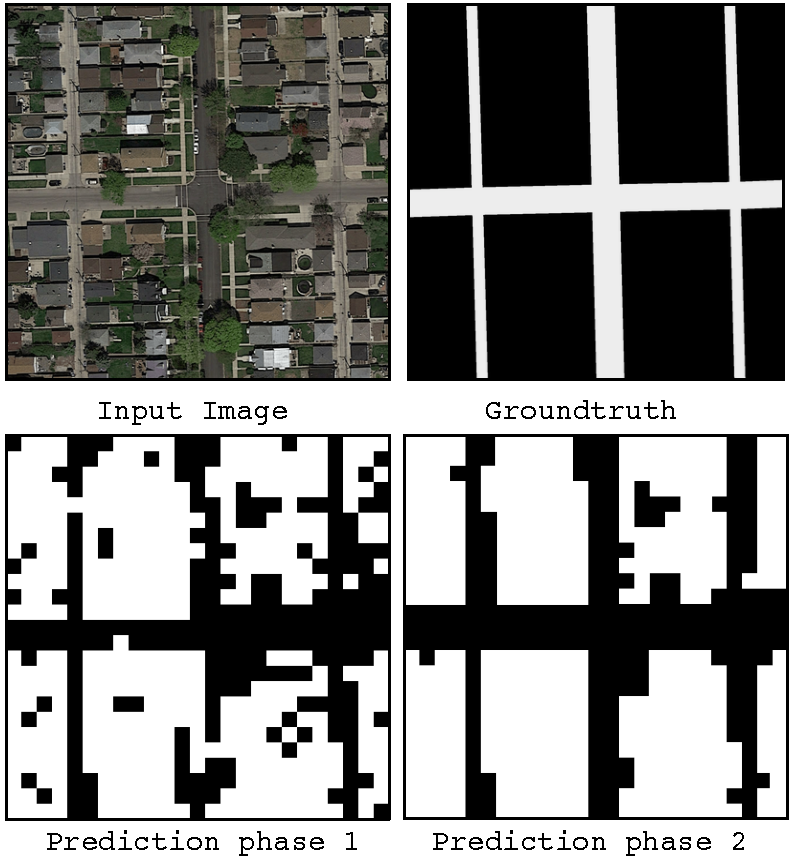
\includegraphics[width=0.35\textwidth]{figures/two_phases_conv2d.pdf}
\caption{\small An example of the application of the two-phase propagation process: for a given input (top-left), the predicted segmentation at output of the neural network (bottom-left) is then re-input to a second neural network trained from groundtruth images (top-right), outputting the final classification (bottom-right).}
\end{figure}


A sample of a possible network architecture (for default parameters) is displayed in figure \ref{fig-conv-2d-architecture}.

\begin{figure*}
\centering
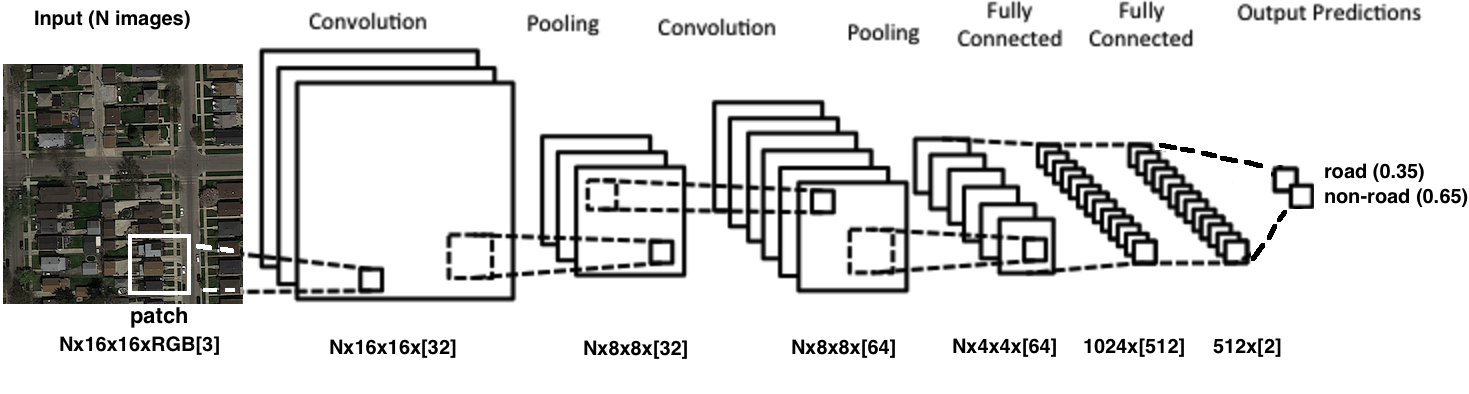
\includegraphics[width=0.9\textwidth]{figures/conv_2d_network.png}
\caption{\small A general overview of the deep network architecture, with default parameters. Dimensionalities, padding types, depths and number of convolution+pooling layers are user-customisable.}
\label{fig-conv-2d-architecture}
\end{figure*}

\section{Results}

\begin{table}
\begin{scriptsize}
\begin{center}

\begin{tabular}{ l r r c l r r }
\hline
\textbf{Dim.} & \textbf{Eigen} & \textbf{Explained} & \hspace{0.1cm} & \textbf{Dim.} & \textbf{Eigen} & \textbf{Explained} \\
    &  \textbf{value} & \textbf{var. ratio} & & & \textbf{value} & \textbf{var. ratio} \\
\hline
\textbf{0} & 1983617.8 & 7.43 e-1 & & \textbf{15} & 3.98 & 1.49 e-6\\
\textbf{1} & 470787.3 & 1.76 e-1  & & \textbf{16} & 3.49 & 1.31 e-6\\
\textbf{2} & 152814.2 & 5.72 e-2  & & \textbf{17} & 2.74 & 1.02 e-6\\
\textbf{3} & 35127.6 & 1.31 e-2   & & \textbf{18} & 2.45 & 9.18 e-7\\
\textbf{4} & 18184.4 & 6.81 e-3   & & \textbf{19} & 1.65 & 6.19 e-7\\
\textbf{5} & 2235.3 & 8.37 e-4    & & \textbf{20} & 1.40 & 5.27 e-7\\
\textbf{6} & 1833.1 & 6.86 e-4    & & \textbf{21} & 0.99 & 3.73 e-7\\
\textbf{7} & 1266.6 & 4.74 e-4    & & \textbf{22} & 0.74 & 2.79 e-7\\
\textbf{8} & 944.0 & 3.53 e-4     & & \textbf{23} & 0.67 & 2.54 e-7\\
\textbf{9} & 519.3 & 1.94 e-4     & & \textbf{24} & 0.61 & 2.30 e-7\\
\textbf{11} & 384.3 & 1.44 e-4    & & \textbf{25} & 0.18 & 6.99 e-8\\
\textbf{10} & 374.8 & 1.40 e-4    & & \textbf{26} & 0.11 & 4.30 e-8\\
\textbf{12} & 178.7 & 6.69 e-5    & & \textbf{27} & 0.05 & 2.17 e-8\\
\textbf{13} & 138.8 & 5.20 e-5    & & \textbf{28} & 0.024 & 9.21 e-9\\
\textbf{14} & 45.78 & 1.71 e-5    & & \textbf{29} & 7.48e-8 & 2.80 e-14\\
\hline
\end{tabular}
\label{table-pca}
\end{center}
\end{scriptsize}
\caption{\small Details on the eigen-vectors after PCA filtering. Features are sorted by relevance (explained variance ratio).}
\label{table-pca}
\end{table}

\paragraph{6. Data Standardization} The final process performs data standardization by subtracting the mean and dividing the values by the standard deviation. This algorithm is particularly helpful to avoid computational overflows. It is only required when PCA is not executed beforehand, as the PCA implicitly executes the standardization.

\section{Machine Learning Methods}
\label{sec-ML}

We implemented the following three least squares methods: \texttt{least\_squares}, \texttt{least\_squares\_GD} and \texttt{least\_squares\_SGD} for least squares with normal equations, regular and stochastic gradient descent. We also implemented \texttt{ridge\_regression} for ridge regression using normal equations, \texttt{reg\_logistic\_regression} for regularized logistic regression using GD and SGD and \texttt{logistic\_regression} for logistic regression with GD and SGD.

Our ideal solution relies on a combination of techniques. To obtain the best results we focus on \textbf{logistic regression}, the only binary classifier, as it provided better results than the available alternative methods. The final pre-filtering consisted of \textbf{mean amputation} over all features and standardization. After that we added a \textbf{polynomial interpolation of the fourth degree} that provided better result compared to the linear counterpart (see accuracy results for different degrees in Table 2). 

\begin{table}
\begin{tabular}{ l l l l | }
Degree & Accuracy (\%) \\
3 & 60 \\
4 & 87 \\
5 & 84 \\
8 & 79 \\
\end{tabular}
\caption{\small Accuracy of predictions on the test data for different degrees of polynomials}
\end{table}

Due to the high amount of computation required, we use logistic regression with \textbf{stochastic gradient descent}.The step size gamma used for gradient descent was found with a binary search across a scope of parameters that yield low time to solution and low loss and set to $1.1e-03$. Finally, we tried to find a better solution using regularized logistic regression and 4-fold cross-validation for obtaining the best lambda. But since the difference between the error in the training data and the error in the test data was negligibly small (see Figure \ref{fig:cross-validation}) we did not pursue the regularized logistic regression further.

\begin{figure}
\centering
%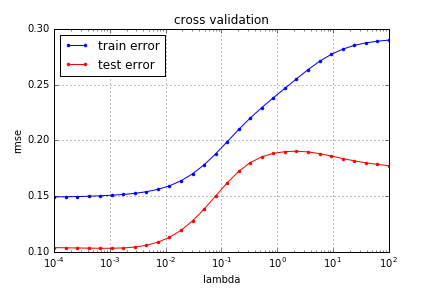
\includegraphics[width=0.47\textwidth]{images/cross_validation.png}
\caption{\small Cross-validation results for test vs training data.}
\label{fig:cross-validation}
\end{figure}

\section{Discussion and Summary}
\label{sec-results}
We applied machine learning techniques to data collected from the CERN particle accelerator aiming at recreating the process of discovering the Higgs particle. We detailed the challenges with the collected data --- many missing values and high dimensionality --- and presented an exploration of pre-filtering and transformation methods for reducing complexity (least significant dimensions) and sample size (outliers), and auto-completion of missing information (mean imputation). We presented the rationale behind an accurate classification based on a combination of algorithms. Our final algorithm can be executed by running \texttt{run.py}. It uses logistic regression with stochastic gradient descent. We cleaned and standardized the data and enriched it by creating a polynomial function of degree 4. This algorithm gave us the following score on Kaggle: $0.81192$ .

%references
\bibliographystyle{unsrt}
\bibliography{report}

\end{sloppypar}
\end{document}